\documentclass[10pt,a4paper]{report}
%\usepackage[latin1]{inputenc}
\usepackage[utf8]{inputenc}
\usepackage{amsmath}
\usepackage{amsfonts}
\usepackage{amssymb}
\usepackage{graphicx}
\usepackage{multicol}
\usepackage{tabularx}
\usepackage{tikz}
\providecommand{\norm}[1]{\left\lVert#1\right\rVert}
\newcommand{\myvec}[1]{\ensuremath{\begin{pmatrix}#1\end{pmatrix}}}
\let\vec\mathbf
%\newcommand{\mydet}[1]{\ensuremath{\begin{vmatrix}#1\end{vmatrix}}}
\usetikzlibrary{arrows,shapes,automata,petri,positioning,calc}
\usepackage{hyperref}
\usepackage{tikz}
\usetikzlibrary{matrix,calc}
\usepackage[margin=0.5in]{geometry}
%\newcommand{\myvec}[1]{\ensuremath{\begin{pmatrix}#1\end{pmatrix}}}
\let\vec\mathbf
\newenvironment{Figure}
  {\par\medskip\noindent\minipage{\linewidth}}
  {\endminipage\par\medskip}
  
  
  
  
\begin{document}
%--------------------logo figure-------------------------%
\begin{figure*}[!tbp]
  \centering
  \begin{minipage}[b]{0.4\textwidth}
   % \includegraphics[scale = 0.05]{iitlogo.jpg}
  \end{minipage}
  \hfill
  \vspace{5mm}\begin{minipage}[b]{0.4\textwidth}
%\raggedleft  \includegraphics[scale = 0.10]{nrc.png}\

  \end{minipage}\vspace{0.2cm}
\end{figure*}
%--------------------name & rollno-----------------------
\raggedright \textbf{Name}:\hspace{1mm} Varsha Reddy\hspace{3cm} \Large \textbf{Assignment-4}\hspace{2.5cm} % 
\normalsize \textbf{Roll No.} :\hspace{1mm} FWC22038\vspace{1cm}
\begin{multicols}{2}

\raggedright \textbf{PROBLEM:}\vspace{2mm}\\
\textbf{ABCD,DCFE and ABFE are parallelograms.Show that   ar(ADE) = ar(BCF)}
\vspace{0.5cm}\raggedright \\
Theory:
Parallelograms on the same base and in between the same parallels are equal in area.\\
Given: ABCD,DCFE and ABFE are parallelograms.
\vspace{2mm} \\ 
%----------------Solution  statement--------------%
\raggedright \textbf{Solution Statement:}\vspace{2mm}
\raggedright \\We can see that the sides of a triangle ADE and BCF are also the opposite sides of a given parallelogram. Now we can show both the triangles are congruent using congruency property. We know that congruent triangles are equal areas.  \\
\vspace{5mm}
%-----------------------------solution---------------------------
\raggedright \textbf{SOLUTION}:\vspace{2mm}\\
parallelogram ABCD  lies  between same parallel lines AD and BC\\
\begin{center}
$\therefore$ AD = BC......(1)\\ 
\end{center}
 parallelogram DECF  lies  between same parallel lines DE and CF\\
\begin{center}
$\therefore$ DE = CF......(2)\\ 
\end{center}
 parallelogram ABEF  lies  between same parallel lines AE and FB\\
\begin{center}
$\therefore$ EA = FB.......(3)\\
\end{center}
\begin{center}
In $\Delta$ADE , $\Delta$BCF\\
$\therefore$ AD = BC \\
$\therefore$ DE = CF \\
$\therefore$ EA = FB \\
$\therefore$ $\Delta$ ADE = $\Delta$ BCF\\

Hence, Proved \\
\
\\
\
\\
\end{center}
\vspace{3mm}
\textbf{Termux commands :}
% \begin{lstlisting}
%python3 matrixline.py
% \end{lstlisting}


The input parameters for this construction are 
\begin{center}
\begin{tabular}{|c|c|c|}
	\hline
	\textbf{Symbol}&\textbf{Value}&\textbf{Description}\\
	\hline
	a&4.5&EA\\
	\hline
	b&4.5&BC\\
	\hline
	c&10&CD\\
	\hline
	d&2.5&DE\\
	\hline
	${\theta}_1$& 25$\pi/180$&$ \angle $BC\\ 
	\hline
	${\theta}_2$& 120$\pi/180$&$ \angle $DE\\ 
	\hline
	${\theta}_3$& 2$\pi/3$&$ \angle $AE\\ 
	\hline
	${\theta}_4$& 35$\pi/180$&$ \angle $CD\\ 
    \hline
	E&$\
	\begin{pmatrix}
		0 \\
		0 \\
	\end{pmatrix}$%
	&Point E\\
	\hline
\end{tabular}
\end{center}

\textbf{To Prove:} 
  \begin{center}
  \begin{equation}
      \vec{Ar(ADE)=Ar(BCF)}
  \end{equation}
  \begin{equation}
      \vec{v1=A-D}
      \end{equation}
      \begin{equation}
      \vec{v2=D-E}
 \end{equation}
 \vspace{3mm}
 Area of the triangle $\Delta$ADE is given by \\
 Ar($\Delta$ADE)
=1/2 x $\norm{\vec{V1}\times\vec{V2}}$
  %\vspace{3mm}
 \begin{equation}
      \vec{v3=B-C}
 \end{equation}
 \begin{equation}
    \vec{v4=C-F} 
 \end{equation}
 \vspace{3mm}
  Area of the triangle $\Delta$BCF is given by \\
  Ar($\Delta$BCF)
  =1/2 x $\norm{\vec{V3}\times\vec{V4}}$
 % \textbf{}
 \end{center}
 \begin{center}
%$\therefore$
\begin{equation}
    \vec{Ar(ADE)=Ar(BCF)}
\end{equation}
\end{center}
 \section{Construction}
  \begin{center}
    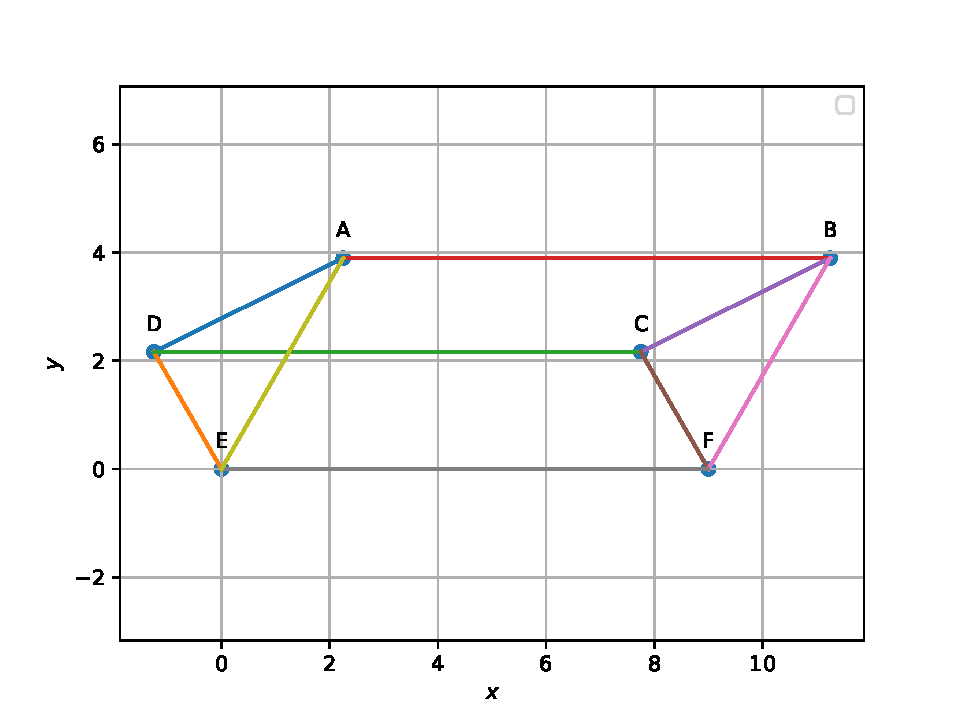
\includegraphics[scale=0.5]{Matrix/ABC.pdf} 
     Figure of Construction
   \end{center}
   \vspace{10mm}
The below python code realizes the above construction: \\
\url{https://github.com/9705701645/FWC/blob/main/lines4.py}

     
\bibliographystyle{ieeetr}
\end{multicols}
\end{document}